In this section, implementation of the control panel is described. The control panel is used to administrate users and devices.
\todo{not enough}

\section{Login}
\begin{figure}[H]
    \centering
    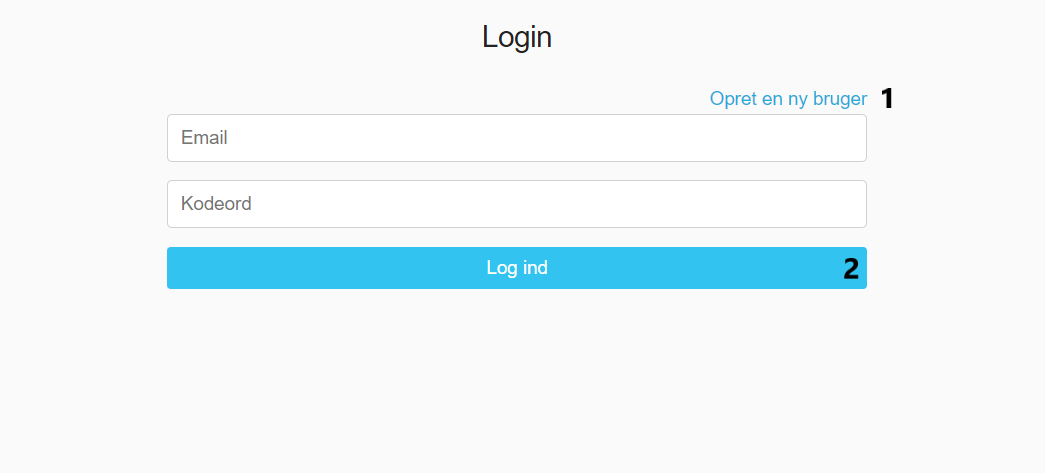
\includegraphics[scale=0.6]{Figures/ControlPanel/LoginView.png}
    \caption{The view presented, when a user should login.}
    \label{fig:controlPanelLoginView}
\end{figure}

When a user tries to first enter the control panel, they will be presented with a login page. A users email and password, are used for authentication. The data is sent as a POST request to \todo{login url missing}. If the authentication is successful, the response is a tuple \todo{example data needed}. If the authentication failed, the response will be a tuple containing the status code 401 for unauthorized and -1 \todo{reason for -1}.


\section{Citizen admin}
\begin{figure}[H]
    \centering
    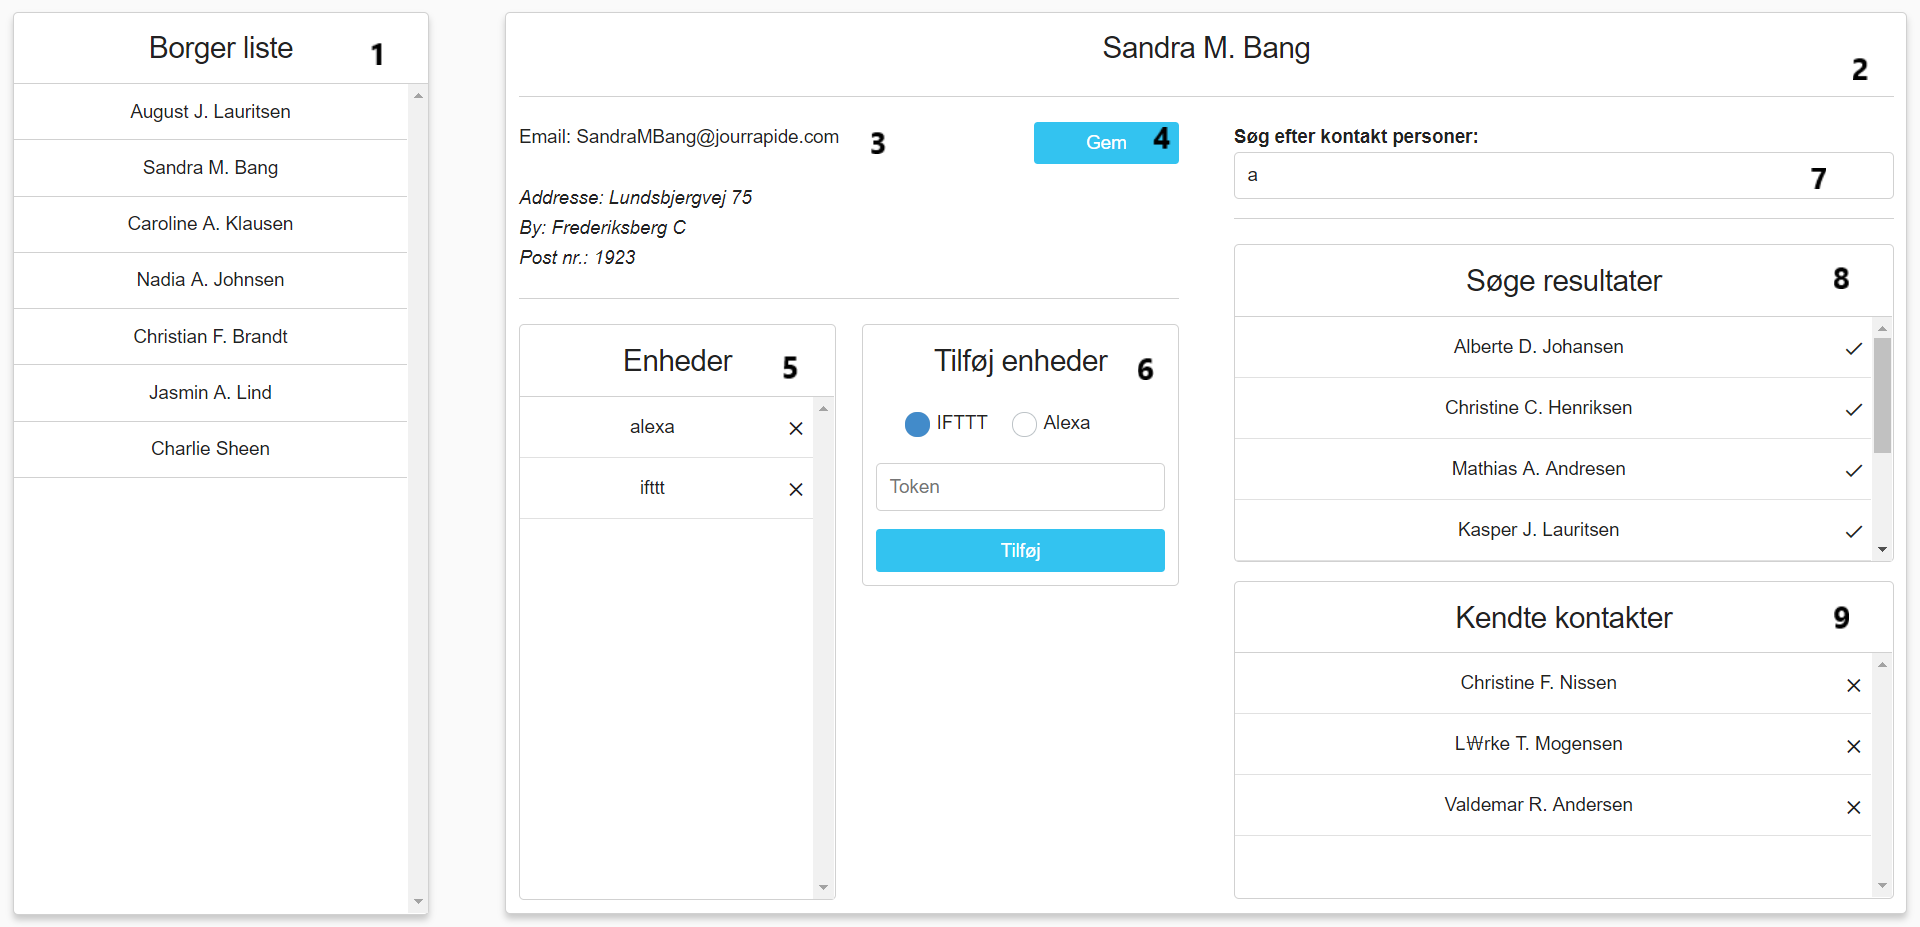
\includegraphics[scale=0.4]{Figures/ControlPanel/CitizenAdminView.png}
    \caption{The view presented for a user, with citizen admin role.}
    \label{fig:controlPanelCitizenAdminView}
\end{figure}

The citizen admin view, is made of three boxes. Box 1 \textit{Tilføj ny borger} is used to add a new citizen, to the logged in citizen admins list of citizens.\\
Box 2 \textit{Borger liste} contains every citizen that the logged in citizen admin, is administrating. When a new citizen is added from box 1, box 2 will be refreshed with the newly added citizen. The fields in box 2, are clickable and will fetch the information for the specific user and will be shown in box 3.

Box 3 presents information for a specific citizen. The box will show the following information:
\begin{itemize}
    \item Full name
    \item Email
    \item Address
    \item City
    \item Postal code
    \item A contact list
\end{itemize}

There is also a search field, where it is possible to search for a phone number that will return a contact if phone number is linked to a contact in our database. There is a button to add that new contact to the contact list. The contact also contains a button to remove a contact. 



\section{Admin}
\begin{figure}[H]
    \centering
    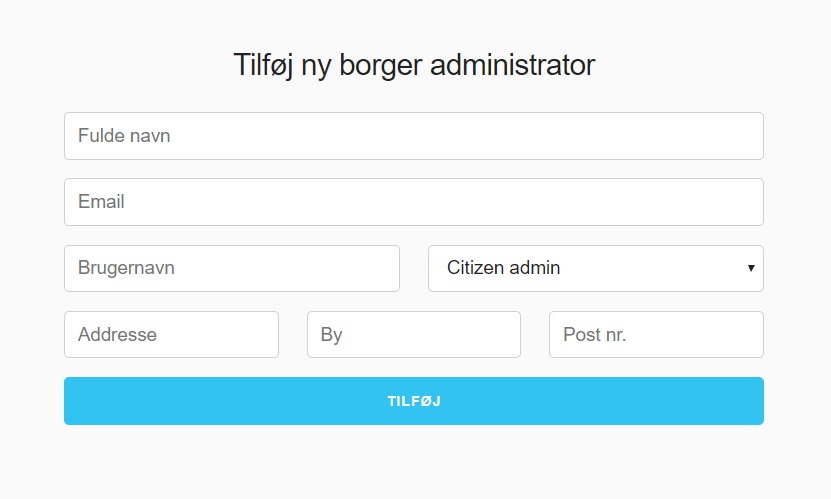
\includegraphics[scale=0.5]{Figures/ControlPanel/AdminView.png}
    \caption{The view presented for a user, with admin role.}
    \label{fig:controlPanelAdminView}
\end{figure}

The admin view \ref{fig:controlPanelAdminView} is very simple. The admin user is only used to add new users of roles citizen and citizen-admin, therefor the view consist of a form that will send a POST request containing the data to \todo{add new user url missing}. \todo{response details}.